\section{Popis jednotlivých součástek a důvody konkrétního tvaru}

\begin{wrapfigure}{R}[0.05\textwidth]{0.7\textwidth}
    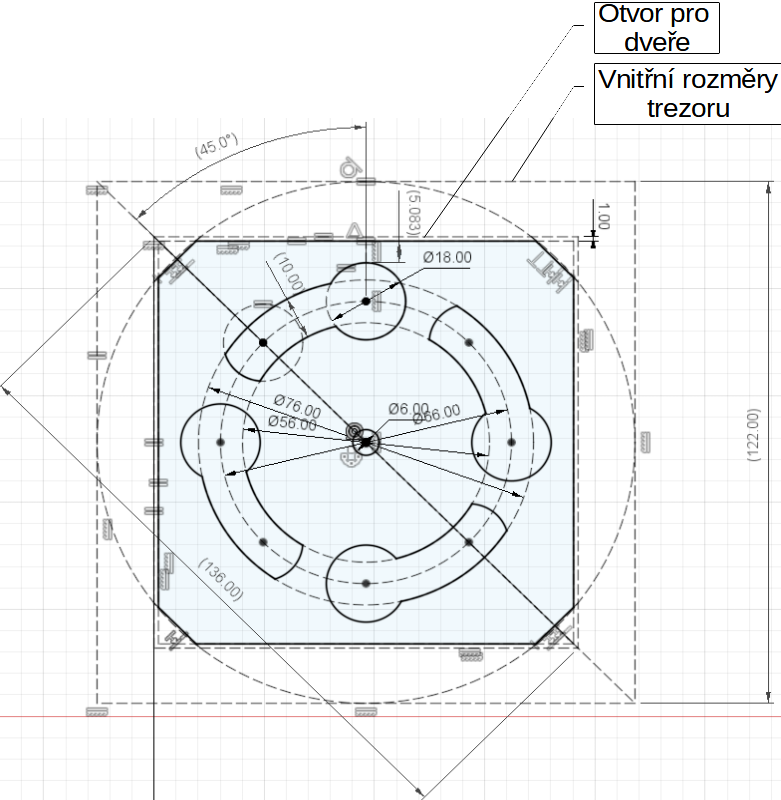
\includegraphics[width=0.7\textwidth]{kapitoly/obrazky/M3/geometrie_zapadky.png}
    \caption{náčrt}
    \label{fig:M3-geometrie-zapadky}
\end{wrapfigure}

\paragraph{Geometrie západky}
Trezor má tvar krychle a délku hrany má 128mm, násobek šestnácti jsem zvolil kvůli jednoduché návaznosti na dřívka, dřevěná dřívka s obdélníkovým průřezem 3x16mm nebo 2x16mm. 
Protože je trezor vyroben z překližky o síle 4mm jsou jeho vnitřní rozměry o 4mm na každé straně menší (takže 122mm). 